% adding the line below for Multifile document support with LatexTools Sublime package 
%!TEX root = manuscript.tex


% Results

\section{Results}

\subsection{Systematic review}

Search terms entered in Pubmed returned 152 results during the last check on December 14, 2017 and 28 articles included in previous
meta-analysis on \gls{nfb} were identified. After the selection process illustrated in \cref{Figure:systematic_review_workflow}, 
31 studies were included in the \gls{saob} and 15 in the meta-analysis as summarized in \cref{Table:table_factors_analysis_meta_analysis_list_studies}.
The 31 studies selected for the \gls{saob} correspond to \citeauthor{Cortese2016}'s criteria to the exception of a need for a control group since 
we are computing the within subject \gls{es}.  

\begin{figure}[h!]
  \centering
  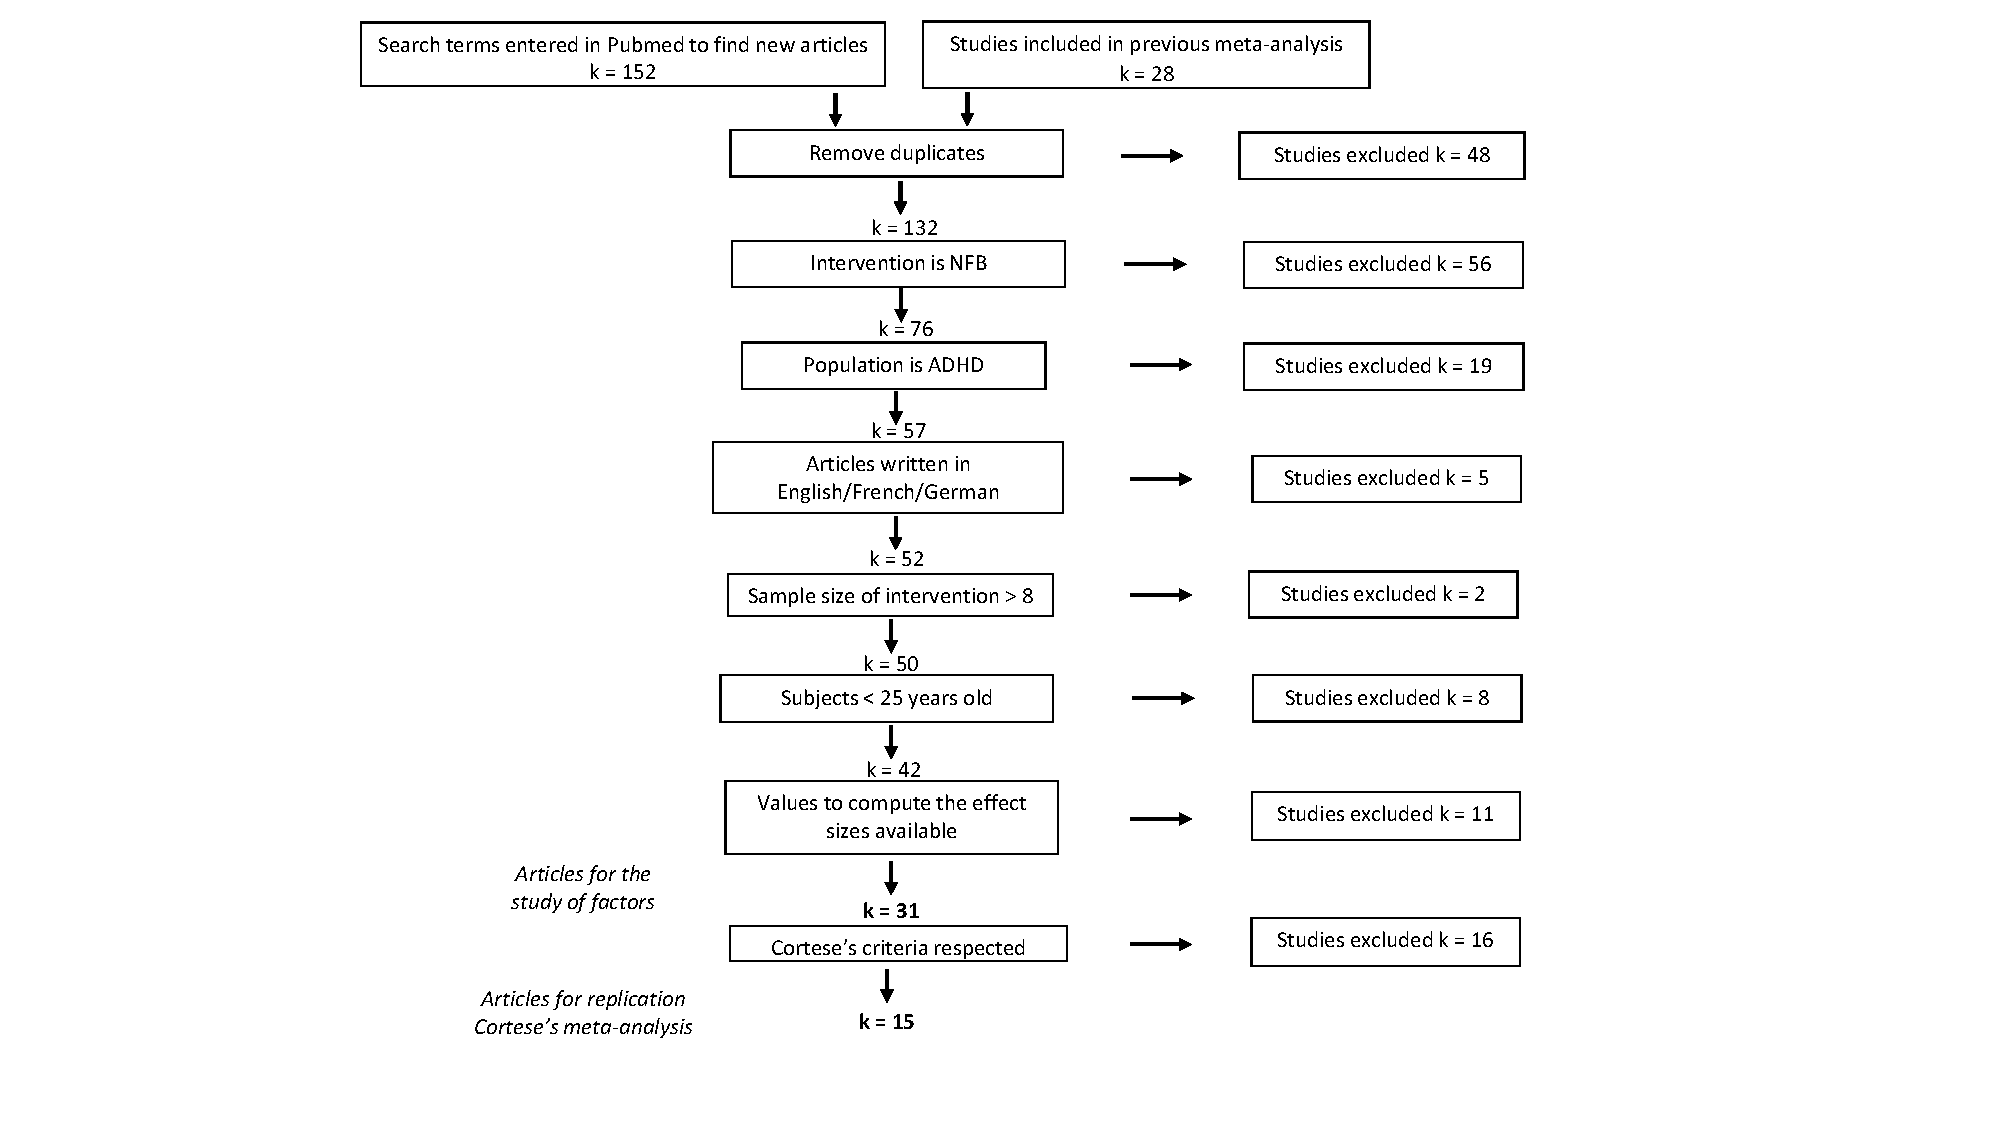
\includegraphics[width=1.0\linewidth]{figures/meta_review_factors_analysis_how_studies_are_included_no_colors_2-columns_fitting_ima}
  \caption{Flow diagram of selection of studies (last search on December 14, 2017). The forlast subset of study exactly corresponds to the 
	studies included in \citet{Cortese2016} and more recent work meeting the same criteria. 
	The last subset ($k$=31) corresponds to the same criteria without the requirement for the presence of a control group.}
  \label{Figure:systematic_review_workflow}
\end{figure}

\begin{table}[h!]
  \centering
  \caption{List of all studies included in the three different analysis. $^a$ Studies originally included in \citet{Cortese2016}
	(search on August 30, 2015), $^b$ studies satisfying \citet{Cortese2016}'s criteria (search on December 14, 2017), $^c$ studies 
	satisfying \citet{Cortese2016}'s criteria to the exception of the part relative to the control group (search on December 14, 2017).}
  \fontsize{9}{11}\selectfont
\begin{tabular}{ cccccc }
\toprule
\multicolumn{3}{ c }{Dataset} & Study & Year & \shortstack{ Size of the \\ \gls{nfb} group } \\
\midrule
 & & & \citeauthor{Arnold2014} & 2014 & 26 \\ 
 & & & \citeauthor{Bakhshayesh2011} & 2011 & 18 \\
 & & & \citeauthor{Beauregard2006} & 2006 & 15 \\
 & & & \citeauthor{Bink2014} & 2014 & 45 \\
 & & & \citeauthor{Christiansen2014} & 2014 & 14 \\
 & & & \citeauthor{Gevensleben2009} & 2009 & 59 \\
 & & & \citeauthor{Heinrich2004} & 2004 & 13 \\
 & & & \citeauthor{Holtmann2009} & 2009 & 20 \\
 & & & \citeauthor{Linden1996} & 1996 & 9 \\
 & & & \citeauthor{Maurizio2014} & 2014 & 13 \\
 & & & \citeauthor{Steiner2011} & 2011 & 9 \\
 & & & \citeauthor{Steiner2014} & 2014 & 34 \\
 & & |\shortstack{ Replicate \\ \citeauthor{Cortese2016}$^a$ } & \citeauthor{VanDongen2013} & 2013 & 22 \\
\cmidrule(lr){3-6}
 & & & \citeauthor{Baumeister2016} & 2016 & 8 \\
 & \shortstack{ Update \\ \citeauthor{Cortese2016}$^b$ } & & \citeauthor{Strehl2017} & 2017 & 72 \\
\cmidrule(lr){2-6}
 & & & \citeauthor{Bluschke2016} & 2016 & 19 \\
 & & & \citeauthor{Deilami2016} & 2016 & 12 \\
 & & & \citeauthor{Drechsler2007} & 2007 & 17 \\
 & & & \citeauthor{Duric2012} & 2012 & 23 \\
 & & &\citeauthor{Escolano2014} & 2014 & 20 \\
 & & & \citeauthor{Fuchs2003} & 2003 & 22 \\
 & & & \citeauthor{Kropotov2005} & 2005 & 86 \\
 & & & \citeauthor{Lee2017} & 2017 & 18 \\
 & & & \citeauthor{Leins2007} & 2007 & 19 \\
 & & & \citeauthor{Li2013} & 2013 & 20 \\
 & & & \citeauthor{Meisel2014} & 2014 & 12 \\
 & & & \citeauthor{Mohagheghi2017} & 2017 & 30 \\
 & & & \citeauthor{Mohammadi2015} & 2015 & 16 \\
 & & & \citeauthor{Monastra2002} & 2002 & 51 \\
 & & & \citeauthor{Ogrim2013} & 2013 & 13 \\
 \gls{saob}$^c$ & & & \citeauthor{Strehl2006} & 2006 & 23 \\
\bottomrule
\end{tabular}

  \label{Table:table_factors_analysis_meta_analysis_list_studies}
\end{table}

\subsection{Replicate a meta-analysis}

The Python module created in order to perform a meta-analysis was successfully validated as describes in the Supplemental Materials and made available online.
So all the following results were computed with the Python code. 

The replication and the following update of \citeauthor{Cortese2016} was conducted by applying the following choices and the results obtained are presented 
in \cref{Table:meta_review_comparison_revman_and_python_with_choices}:

\begin{itemize}
    \item to compute the \gls{es} for \citet{Arnold2014}, \citet{Cortese2016} took as post-test values the assessments after 12 \gls{nfb} sessions
		because results at post-test were not available. In our case, we use the values at post-test (i.e after the 40 sessions). With these values, 
		we find smaller \gls{es} than \citet{Cortese2016};  
    \item different results for teachers' assessments are found for \cite{Steiner2014} because we decided not to use the same scale 
		as \citeauthor{Cortese2016}. Indeed, \citeauthor{Cortese2016} relied on the BOSS Classroom Observation \citep{Shapiro2010} to compute \gls{es}
		for teachers' ratings even if this scale is not as used as other scales provided in this study. That's why we decided to conduct our analysis
		with a more common scale which has been part of studies assessing the pros and cons of different ADHD scales \citep{Epstein2012, Collett2003}: The Conners. 
		Besides, this scale is already used in this study to compute the \gls{es} for the parents' ratings. 
		Using this scale leads to higher \gls{es} in attention but not in total and hyperactivity. Moreover, this different choice of 
		scale does not affect the significance of the summary effects.
\end{itemize}

\begin{table}[h!]
  \centering
  \caption{Comparison between \citet{Cortese2016} results obtained with RevMan \citep{RevMan} and those obtained with the Python code with our 
	choices applied. Summary effects and their corresponding p-value (in parenthesis) are presented. With the Python program, a negative \gls{se}
	is in favor of \gls{nfb}.}
\begin{tabular}{cccc}

\toprule
\multicolumn{2}{c}{Input data} & \shortstack{ Results from \\ \citet{Cortese2016} \\ (for reference)} & \shortstack{ Means and standard \\ deviations from \\ articles included in \\ \citet{Cortese2016} }\\
\midrule
\multicolumn{2}{c}{Implementation} & \shortstack{ RevMan \\ \citet{RevMan} } & Python program\\
\midrule
\multicolumn{2}{ c }{Hypothesis} & \shortstack{ Same as \\ \citet{Cortese2016} } & Our choices$^a$\\
\midrule
\multirow{ 3}{*}{ \textit{Parents} } & Total & $0.35$ ($0.004$) & $-0.32$ ($0.013$)\\
 & Inattention  & $0.36$ ($0.009$) & $-0.31$ ($0.036$)\\
 & Hyperactivity  & $0.26$ ($0.004$) & $-0.24$ ($0.02$)\\
\multirow{ 3}{*}{ \textit{Teachers} } & Total & $0.15$ ($0.20$) & $-0.11$ ($0.37$)\\
 & Inattention  & $0.06$ ($0.70$) & $-0.17$ ($0.16$)\\
 & Hyperactivity  & $0.17$ ($0.13$) & $-0.022$ ($0.85$)\\
\bottomrule

\end{tabular}

  \label{Table:meta_review_comparison_revman_and_python_with_choices}
\end{table}

Consequently, the rest of this work was carried with the following choices:
\begin{itemize}
    \item values used to compute \gls{es} from \citeauthor{Arnold2014} correspond to the scores at post-test (after the 40 sessions of \gls{nfb};  
    \item to compute the \gls{es} based on teachers' assessments, we used the Conners because this scale is more common.
\end{itemize}

\subsection{Update a meta-analysis}

The next step consists in extend \citeauthor{Cortese2016} meta-analysis by adding the two new articles \citep{Strehl2017, Baumeister2016} found 
during the systematic review. \citet{Baumeister2016} provides results only for parents total outcome whereas \citet{Strehl2017} gives teachers 
and parents' assessments for all outcomes. In spite of favorable results for \gls{nfb}, particularly on parents' assessments, adding these two 
new studies does not change either the magnitude or the significance of the \gls{se} for any outcome whatever the raters
as illustrated in \cref{Figure:meta_review_forest_plots_update_meta_analysis_our_choices_no_colors_2-columns_fitting_image}. 
 
\begin{figure}[h!]
  \centering
  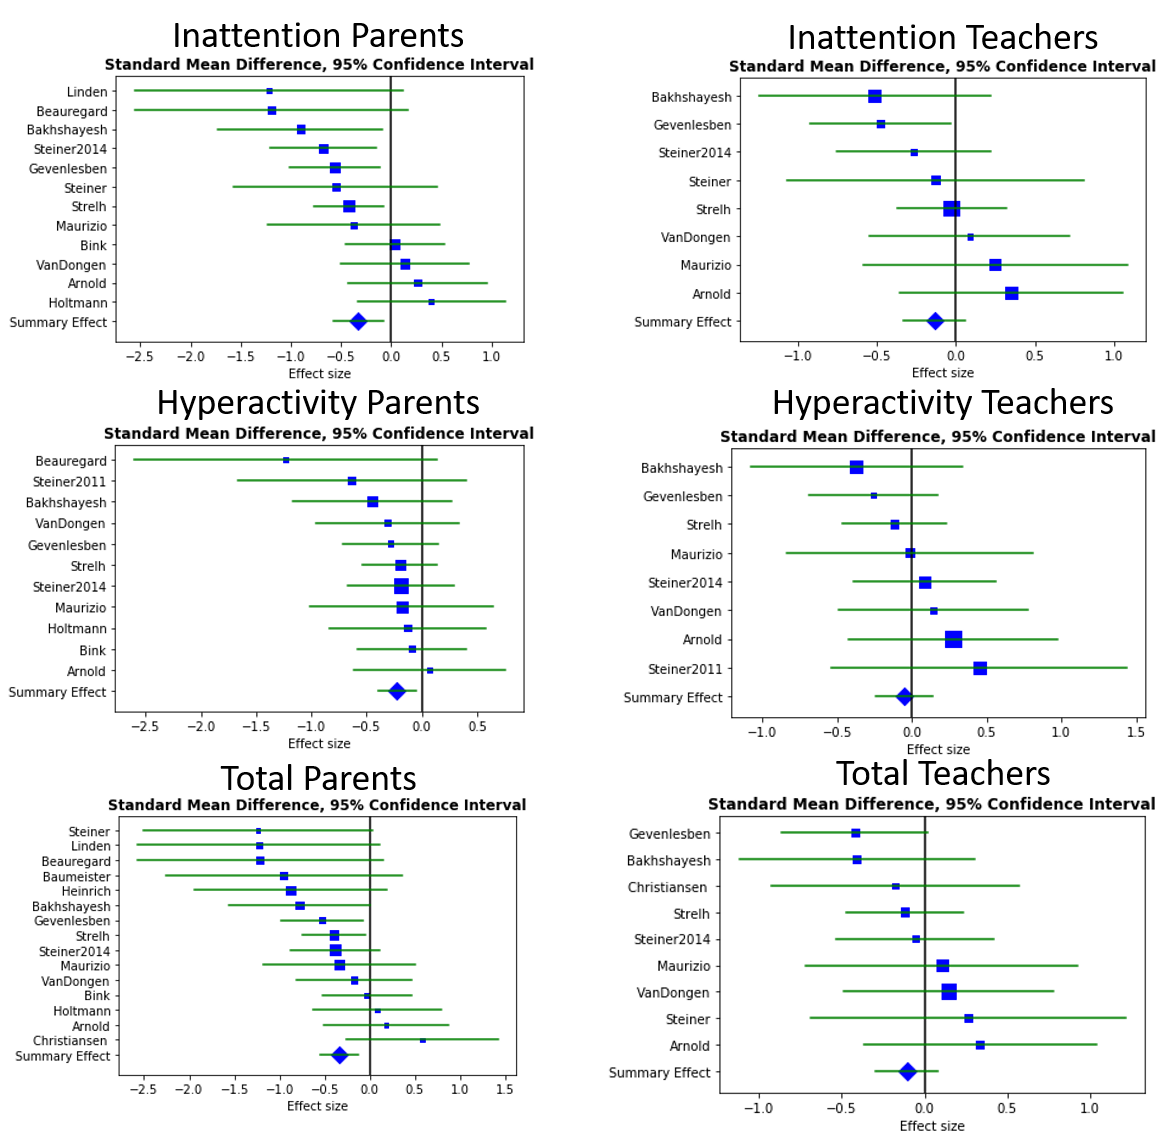
\includegraphics[width=1.0\linewidth]{figures/meta_review_forest_plots_update_meta_analysis_our_choices_no_colors_2-columns_fitting_image}
  \caption{Forest plots obtained on the dataset "Update meta-analysis" with the Python code. A negative \gls{es} is in favor of \gls{nfb}. 
	The blue squares correspond to the \gls{es}, the blue diamond to the \gls{se} and the green line to the confidence interval.}
  \label{Figure:meta_review_forest_plots_update_meta_analysis_our_choices_no_colors_2-columns_fitting_image}
\end{figure}

Next, we run the analysis on two specific subgroups: on the one hand only studies following standard protocol defined by \citet{Arns2014}
are selected and on the other hand only studies forbidding participants to take medication during the clinical trial are included. 

Regarding the standard protocol subgroup, \citet{Cortese2016} found all the outcomes significant except for the hyperactivity symptoms 
rated by teachers. However, when adding \citep{Strehl2017} results, we find no significance for the inattention symptoms assessed by 
teachers as well (p-value = 0.11). 
As for the low/no medication subgroup, summary effects are not significant except for the inattention symptoms assessed by parents (p-value = 0.013). 
Besides, the differences in \citet{Arnold2014} values causes a loss of significance in 
hyperactivity outcome for parents (p-value = 0.066) compared to \citet{Cortese2016} (p-value = 0.016). The two new studies are not 
included in this subgroup because subjects are taking psychostimulants during the trial.

All the scales used to compute the effect sizes following our choices are summarized in the Supplemental Materials.

\subsection{Detect factors influencing the Neurofeedback}

This analysis is performed on 31 trials assessing the efficacy of \gls{nfb} as presented in \cref{Table:table_factors_analysis_meta_analysis_list_studies}. 
Among the 25 factors selected, 6 are removed because there are either too many missing observations or they were too homogeneous: beta up frontal, 
the use of a transfer card, the type of threshold for the rewards (incremental or fixed), the EEG quality equal to 3 and presence of a control group. 

The \gls{es} within subjects is computed for all available clinical scales of each study and then factors are associated with the computed \gls{es}
thanks to three different methods: the \gls{wls}, the \gls{lasso} and the decision tree. The global results are presented in \cref{Table:table_factors_analysis_results_summary}
where we observe that the techniques used do not return exactly the same factors. Thus, the more methods identified a factor, the more confident we can be in
the results.  

\begin{table}[h!]
  \centering
  \caption{Results of the \gls{wls}, \gls{lasso} and decision tree. For the \gls{wls}, a p-value $<$ 0.05 (in bold) means that the coefficient of 
	the corresponding factor is significantly different from 0. For the \gls{lasso}, factors not set to 0 (in bold) are selected. 
	When the value of the coefficient is negative, the corresponding factor may lead to better \gls{nfb} results.}
  \begin{center}
\begin{tabular}{ p{3cm} p{3cm} p{3cm} p{2cm} p{2cm} p{2cm}}
\toprule
\multicolumn{2}{c}{ \shortstack{Independent \\ variables (factors)} } & \shortstack{ \gls{wls} \\ (p-value) } & \gls{lasso} & \shortstack{Decision \\ Tree} \\
\midrule
\multirow{ 2}{*}{ \textit{Signal quality} } & \gls{eog} correction & \hskip 0.08in-0.078 (0.41) &  \hskip 0.12in0.00 & / \\ 
& artifact correction based on amplitude & \hskip 0.12in\textbf{0.15(0.040)} & \hskip 0.12in\textbf{0.047} & / \\ 
\midrule
\multirow{ 3}{*}{ \textit{Methodological} } & \gls{pblind} & \hskip 0.12in\textbf{0.10 (0.043)} & \hskip 0.12in\textbf{0.11} & \textbf{selected} \\ 
& randomization & \hskip 0.12in0.0069 (0.92) & \hskip 0.12in\textbf{0.032} & / \\  
& \gls{irb} & \hskip 0.08in\textbf{-0.29 (0.00)} & \hskip 0.08in\textbf{-0.15} & / \\  
\midrule
\multirow{ 3}{*}{ \textit{Population} } & age max & \hskip 0.08in-0.090 (0.16) & \hskip 0.12in0.00 & / \\
& age min & \hskip 0.08in-0.055 (0.37) & \hskip 0.12in0.00 & \textbf{selected }\\
& on drugs & \hskip 0.12in0.069 (0.42) & \hskip 0.12in\textbf{0.032} & / \\
\midrule
\multirow{ 9}{*}{ \textit{ \shortstack{\gls{nfb} \\ implementation} } } & number of sessions  & \hskip 0.08in-0.0075 (0.92) & \hskip 0.12in0.00 & / \\
& session length & \hskip 0.12in0.17 (0.17) & \hskip 0.12in0.00 & \textbf{selected} \\
& treatment length & \hskip 0.12in\textbf{0.57 (0.00)} & \hskip 0.12in\textbf{0.33} & \textbf{selected} \\
& session pace & \hskip 0.08in\textbf{-0.25 (0.00)} & \hskip 0.08in\textbf{-0.14} & / \\ 
& \gls{smr} & \hskip 0.08in-0.063 (0.41) & \hskip 0.12in\textbf{0.061} & \textbf{selected} \\
& beta up central & \hskip 0.08in-0.027 (0.72) & \hskip 0.12in0.00 & / \\  
& theta down & \hskip 0.08in\textbf{-0.29 (0.014)} & \hskip 0.08in\textbf{-0.051} & / \\
& \gls{scp} & \hskip 0.08in-0.099 (0.50) & \hskip 0.12in\textbf{0.10} & / \\ 
& transfer phase & \hskip 0.12in\textbf{0.27 (0.032)} & \hskip 0.12in\textbf{0.11} & / \\
\midrule
\multirow{ 2}{*}{ \textit{ \shortstack{Quality of \\ acquisition} } } & more than one active electrode & \hskip 0.12in0.064 (0.36) & \hskip 0.12in0.00 & / \\ 
& \gls{eeg} quality 2 & \hskip 0.08in\textbf{-0.36 (0.00)} & \hskip 0.08in\textbf{-0.23} & \textbf{selected} \\  
\bottomrule
\end{tabular}
\end{center}

  \label{Table:table_factors_analysis_results_summary}
\end{table}

First, after applying the \gls{wls}, we find that 8 factors are significantly different from zero for an adjusted R-squared of 0.74. 
When applying the \gls{ols}, the same factors are returned as significant except the transfer phase, the protocol theta down and the artifact correction
based on amplitude with an adjusted R-squared of 0.42. The \gls{lasso} regression selects significant factors by setting to 0 the others: 12 factors 
are different from 0 here. With these two methods, a negative coefficient means that the factor is in favor of the \gls{nfb}.

Eventually, the decision tree presented in \cref{Figure:factors_analysis_decision_tree_results} splits the dataset based on the factor leading to the
smallest \gls{mse}. The best predictor is the one at the top of the tree: in our case it is the \gls{pblind}. Five other factors also splits the subsets. 

\begin{figure}[h!]
  \centering
  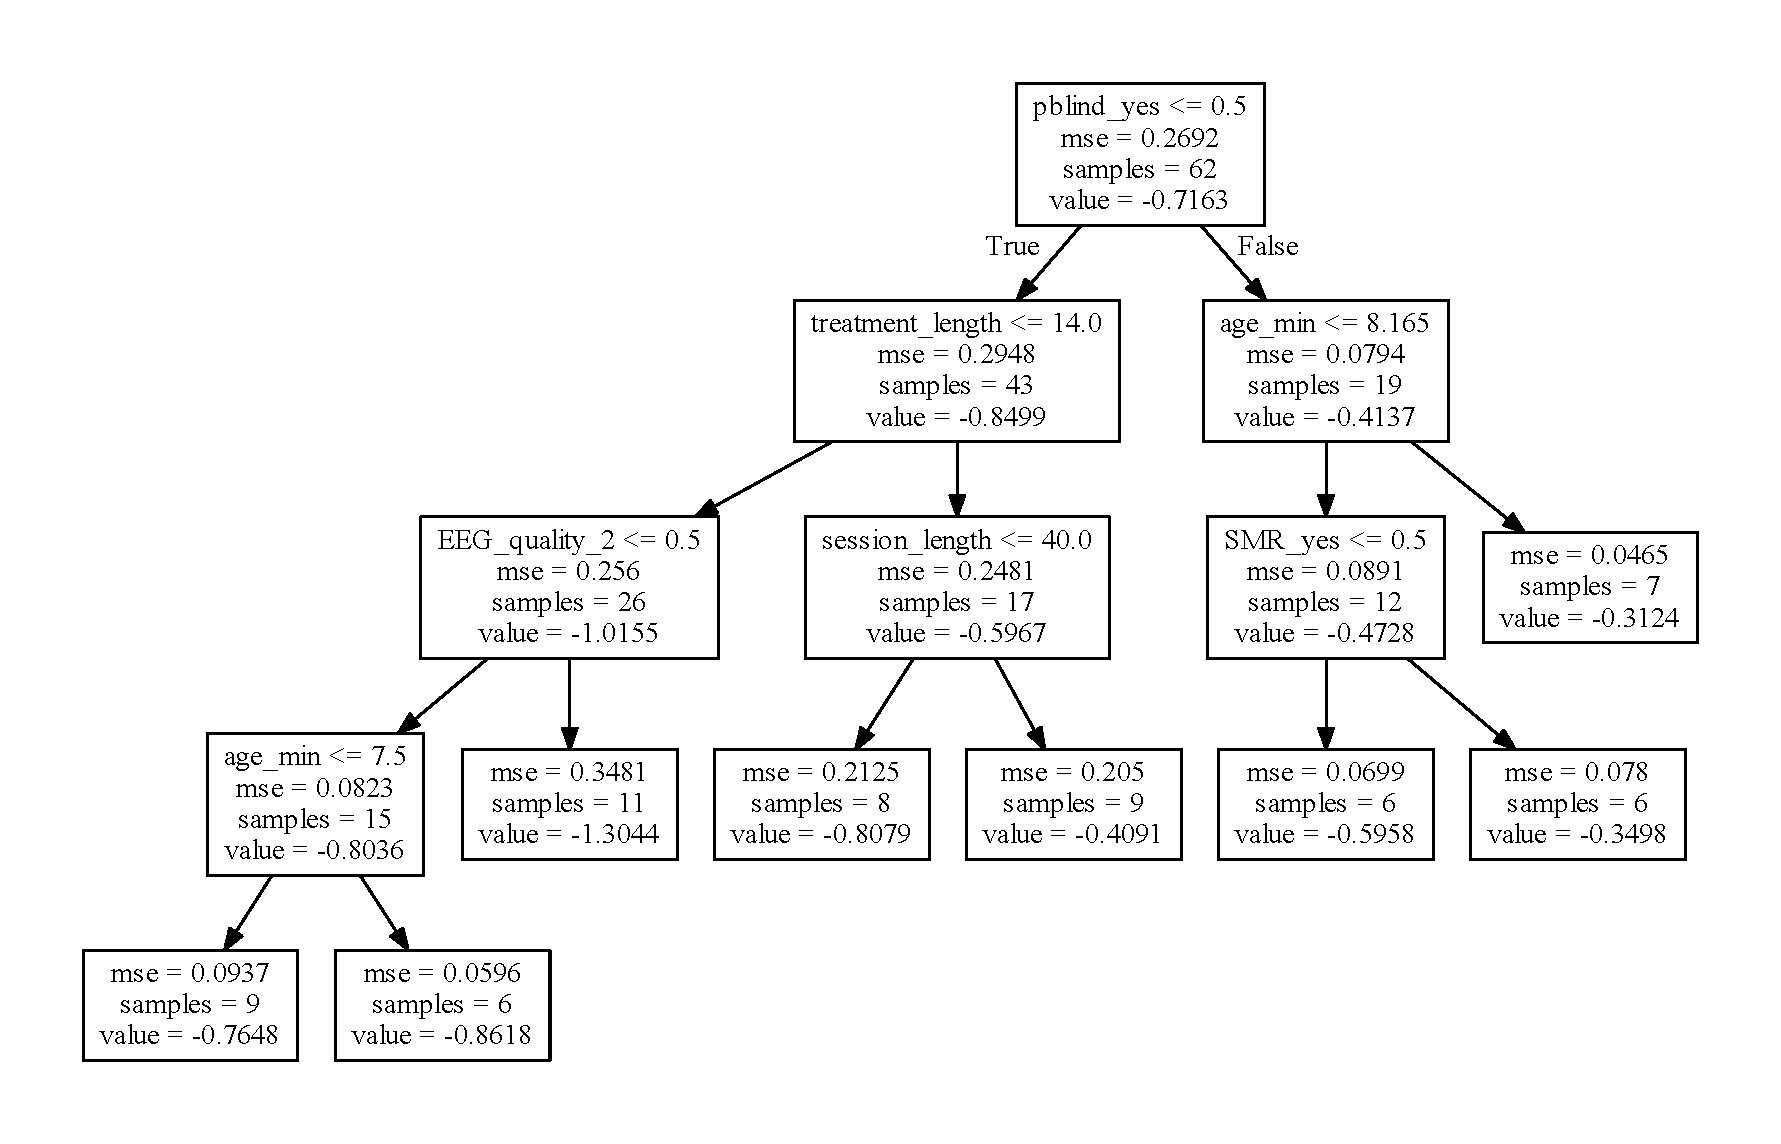
\includegraphics[width=1.0\linewidth]{figures/factors_analysis_decision_tree_results_no_colors_2-columns_fitting_image}
  \caption{Decision Tree obtained with the factors. The criteria to minimize was the \gls{mse}. For the dummy variables, a value of $1$ means
	that the factor is observed in the study. The value corresponds to the dependent variable.}
  \label{Figure:factors_analysis_decision_tree_results}
\end{figure}

We can notice that several factors are common to the three methods, in particular the treatment length, the assessment 
by a blind rater and \gls{eeg} quality of 2 which are returned by the three methods. Besides, 
the methods agree on the direction of the influence of these factors. However, it is more difficult to interpret the influence of the factors 
returned only by one or two methods. For instance, both \gls{wls} and \gls{lasso} find that  
relying on the amplitude of the signal to correct artifacts, and including a transfer phase seem not to improve the \gls{adhd} symptoms. 
Conversely, the \gls{irb} approval, a theta down protocol, and a high number of sessions per week appear to 
positively influence the results. The decision tree and \gls{lasso} have in common the protocol \gls{smr}: it is associated with lower \gls{es}.
Five factors are returned by only one of the methods: the minimal age of the children, being on drugs 
during \gls{nfb} treatment, randomizing the groups and the \glspl{scp} protocol. 

%A negative coefficient means that the factor is in favor of the \gls{nfb}. Here, among the factors whose coefficient is significantly 
%different from 0, a long treatment, a blind rater, including a transfer phase, and correcting artifact thanks to the amplitude appear 
%to have a negative influence on the \gls{nfb} performance. Conversely, an \gls{irb} approval, a high number of sessions per week, a theta
%down protocol and an EEG quality of 2 seem to lead to more efficacy. 

%With this method, a negative coefficient corresponds also to favorable factors. Thus, having several sessions per week, being approved 
%by an \gls{irb}, a protocol theta down, and an EEG quality of 2 seem to improve the results of the \gls{nfb}. 
%On the contrary, a blind rater, a long treatment, randomizing the groups, a \glspl{scp} and \gls{smr} protocols, being on drugs during the trial, correcting 
%artifact based on the amplitude of the signal, and including a transfer phase during the session appear to be factors with a negative influence.

 

%So, the dataset is divided in two subsets: 
%43 samples where the assessments were reported by non-blind raters and 19 samples based on blind ratings. This last subset, where the \gls{se} is smaller 
%than the one obtained for non-blind raters, is split on the age min criteria: it appeares that the lower the age, the better the results. Regarding 
%the side of the tree where the raters are non-blind, the next factor leading to the smallest \gls{mse} is the treatment length. A smaller treatment
 %length seems to lead to better \gls{nfb} results. In that case, the EEG quality 2 enables to break down the subset and according to these results
 %if this factor is respected in studies it seems to lead to higher \gls{se}. The lower we get into the tree, the less samples are available, so results 
%were less and less reliable.

 

% words number = 1635
